%% ----------------------------------------------------------------
%% Hardware Development.tex
%% ---------------------------------------------------------------- 
\chapter{Initial Hardware and Firmware Development} \label{Chapter:HardwareDevelopment}
For initial development, the \textit{Il Matto} board, designed by Steve Gunn, was used. The system has an ATMega644P clocked at 12MHz and has an on-board SD card socket. 

The following section is broken down into the following parts:
\begin{enumerate}
\item Camera Code
\item SD Card
%\item Motor Control
\item Circuit and PCB Development
\end{enumerate}

\section{Camera} \label{Section:Camera}

The camera used is an OV7670 by OmniVision. It is mounted onto a break out board and connected to a AL422B FIFO Buffer. The breakout board has all passive components needed and a 24MHz clock mounted. The schematic for the device can be seen in appendix \ref{Chapter:AppendixA:CircuitDiagrams}.

Original code for the camera operation was given by Steve Gunn, which I used to gain the operation required. This code streamed continuous video to a TFT screen. The operation required was to take a single photo from the camera and store the data. 

\subsection{Single Camera Operation}

The camera uses a SCCB Interface \citep{SCCB_Interface} created by OmniVision. This is almost identical to the $I^{2}C$ Interface by Phillips and the two protocols are compatible. The original code used a bit-banged SCCB interface which was very slow and used up processing time. This was changed to make used of the built-in interrupt-driven $I^{2}C$ interface (named TWI in Atmel AVRs)\footnote{$I^{2}C$ , SCCB and TWI are all the same but are called differently due to Phillips owning the right to the name ``$I^{2}C$"}. This communication bus is used to set up the control registers of the OV7670 to enable operation in the correct format. RGB565 is used in my application.

RGB565 is a 16 bit pixel representation where bits 0:4 represent the blue intensity, 5:10 is the green intensity and 11:15 represent the red intensity (see figure \ref{fig:RGB565}). This is a compact way of storing data but only allows 65536 colours. Greys can also appear to be slightly green due to the inconsistent colour ratio of the green field. 
\begin{figure}
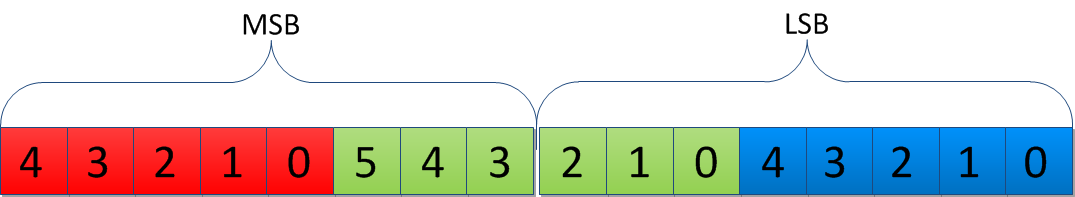
\includegraphics[width = \textwidth]{./Figures/RGB565.png}
\caption{RGB565 pixel format}
\label{fig:RGB565}
\end{figure}

The camera must use a high speed clock in order to ensure the pixels obtained are from the same time. This makes it difficult for an AVR to be able to respond to the camera quick enough (ATMegas typically clocked at 8-12MHz). This highlights the necessity for a FIFO Buffer. 

The OV7670 is set up so that the VSYNC pin goes low at the beginning of every full frame of data, and HREF is high when the data being output is valid. The pixel data is then clocked out on every rising edge of PCLK. To control the buffer, WEN (write enable) is NAND with the HREF signal. When both are high, the write enable to the buffer will be active and the data will be clocked in by PCLK. In order to acquire a full frame, the first VSYNC pin is set up to interrupt the AVR to enable WEN. The camera will output an entire frame of pixel data and store it into the buffer. When the second VSYNC is received, the WEN signal is disabled, stopping any more data being stored. The FIFO buffer now contains an entire image.

To obtain the data from the buffer, the AVR sets output enable and pulses the read clock. Valid data is available on the input port while RCLK is high. All the data is then read in half a pixel at a time. The entire operation can be seen in figure \ref{fig:ov_Capture}.
\begin{figure}
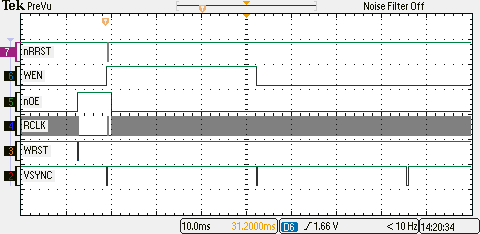
\includegraphics[width = \textwidth]{./Figures/ov7670_im_capture.png}
\caption{Signals generated to control the OV7670 capture and read}
\label{fig:ov_Capture}
\end{figure}


Difficulties arose at this point with the storage of the data. The ATMega644P has 4kB of internal SRAM, but  153.6kB of memory is needed to store a single image at QVGA (320 by 240 pixels, 2 bytes per pixel) quality. 

Firstly, data was sent straight to a desktop computer via a COM Port using USART. A simple desktop program was written in C\# to receive and store all the data, and to make a Bitmap image from the data. This method was slow, taking around 30 seconds to transmit one uncompressed image. 

The second option was to use extra memory connected to the microcontroller. An SD card is used as FAT file system so that data can be looked at by a user on a computer. Text log files are also written to aid debugging. This is discussed in section \ref{sect:SDCard}. 

\subsection{Dual Camera Operation}
In order for stereovision to be successful, two cameras separated by a horizontal distance ($B$) will need to be driven at the same time to obtain photos within a small time frame of one another.

A major problem occurred with using the \itc interface to set up both cameras. The camera has a set \itc address of $21_{16}$, which cannot be changed. Multiple \itc devices with exactly the same address cannot be used on the same bus. 
Two solutions to this are possible: driving one from $I^{2}C$ and one from SCCB, or using an \itc multiplexer. By using two different buses, there can be no bus contention. However, SCCB is slow and processor-hungry as it deals with the protocol bit by bit in software. This takes up memory and is not reusable for other operations.

An \itc multiplexer sits on the bus and has multiple output buses. The master can then address the multiplexer and select whether to pass the bus to bus 0, bus 1 or not allow the data to be transferred. This saves processor time, but means a write operation has to be done to select the camera bus before being able to write to the camera. This slows down the operation, but not as much as using SCCB. The main disadvantage to the \itc MUX is the extra hardware needed; firstly the MUX itself, but also 7 extra resistors to pull up the two extra buses and the three interrupt lines must be added. 

Overall, the disadvantages posed by using a MUX are small, so a multiplexer will be used as opposed to the SCCB interface. A suitable multiplexer is the Phillips PCA9542A \citep{I2C_Mux}.

The buffers have an output enable pin so the data bus can be shared by both cameras to the AVR. The ATMega644P offers three interrupt pins, two of which are used by the two VSYNC pins for the cameras.

Two ISRs are used to control the VSYNC signals, and when taking a photo, both frames are taken at a time period close together to capture the same scenario. The data for both images are read back individually by the AVR. 

Operation to read an image is identical to using one camera. However, an ID number is passed through the functions to make a decision on the pins to use to read the buffer and to enable the output. Care was taken to avoid bus contention, but no checking procedure is explicitly in place. Both images are then read back from the buffers and stored to memory. 

\section{SD Card} \label{sect:SDCard}

To use the SD card, the FATFS library \citep{FATFS} was used. The library supplies all the functions for writing a FAT File System in the files \textit{ff.c}, \textit{ff.h}, \textit{ffconf.h}, \textit{diskio.c}, \textit{diskio.h} and \textit{integer.h}. The \textit{diskio.h} functions control what device is being used - SD/MMC Card, USB drive etc. The \textit{ff.h} header contains all the functions to write to in a FAT File system. 
\\
An SD card was chosen due to it's small size, low cost and a large data storage. The cards work using an SPI bus which can be used for other devices within the system so the card only uses one extra enable pin in hardware to function. 

\subsection{Storing Images}

Many image formats are common, such as Joint Photographic Expert Group (JPEG), Portable Network Graphics (PNG), Bitmap (BMP) and Graphics Interchange Format (GIF). Table \ref{ImageFormats} shows a summary of some common image formats.


\begin{table}
\centering
\begin{tabular}{|p{3cm}| p{2cm}|p{2cm}|p{2cm}|p{2cm}|} \hline
			&	Bitmap 		& 	JPEG			 	&	PNG				& 	GIF \\ \hline
Extension 		& 	*.bmp 		&  	*.jpg /*.jpeg 		& 	*.png				& 	*.gif \\ \hline
Compression 	& 	No 			& 	Lossless  and Lossy		&	Lossless ZIP			&	Lossy	\\\hline
File Size of 320 by 
240 pixel Image (kB) &	225			&	20				&	23				&	24 \\\hline
Bits per Pixel		&	8, 16, 24 or 32	&	24				&	24, 32 or 48 			& 	24, but only 256 Colours \\


\hline
\end{tabular}
\caption{A table comparing different image formats available (\cite{ImageComparison})}
\label{ImageFormats}
\end{table}

It is clear that the best choice for images would be either PNG or JPEG. However, these require more computational time to compress the image into the correct format. To avoid compression, and thereby save processing time, bitmap was chosen at the expense of using more memory. The data in a bitmap image is also stored in RGB format so can be read back easily when processing the image. Appendix \ref{Chapter:AppendixB:BMPFile} shows the make up of a Bitmap File that was used.

By writing the image in this format, they are then able to be opened on any operating system. This aids debugging and allows the prototyping of image algorithms in a more powerful environment. Figure \ref{ExampleImage} shows a photo taken by the OV7670 and stored on a SD card.

\begin{figure}
\begin{center}
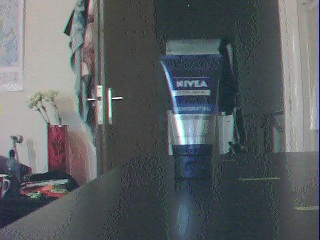
\includegraphics{Figures/ExampleImageFromCamera.jpg} 
\end{center}
\caption{An Example Image taken using the OV7670 and stored as a Bitmap on the SD Card}
\label{ExampleImage}
\end{figure}

\subsection{User Interface}
The ATMega 664P pinout for the dual camera operation can be seen in table \ref{table:644Pin}. Due to a lack of available GPIO pins, an ATMega168 was added on the \itc bus to act as a port extender. The ATMega168 accepts a read or write command. A write places the written data on Port D and a read returns any button pressed that occurred on Port C. When a button is pressed, this is stored in the ATMega168 until a read has been done. This is so the master (644P) does not miss any button presses while busy doing lengthy operations such as writing an image. The code is based on Application Note AVVR311 \citep{Atmel:I2CSlave}, written for IAR Compiler. This code was altered to compile with GCC under Atmel Studio. AVRs contain a hardware based \itc protocol that is interrupt based in software. The interrupt service routine of the TWI vector is a state machine which loads the data to send, stores received data, responds to acknowledges and address calls and deals with bus errors that can occur.

\begin{table}
\centering
\begin{tabular}{|c|c|c|c|c|}\hline
	& 	Port A 	& 	Port B 			& 	Port C 				& 	Port D 		\\ \hline
0	&	Data 0	&	SD Write Protect&	\itc - SCL			&	No Connection	\\
1	&	Data 1	&	SD Card Detect	&	\itc - SDA			&	No Connection	\\
2	&	Data 2	&	USB Data Plus	&	Read Clock 1		&	VSync 0			\\
3	&	Data 3	&	USB Data Minus	&	Read Reset 1		&	VSync 1			\\
4	&	Data 4	&	SPI Chip Select	&	Write Enable 1		&	Read Clock 0	\\
5	&	Data 5	&	SPI	MOSI 		&	Write Reset 1		&	Read Reset 0	\\
6	&	Data 6	&	SPI MISO		&	Output Enable 0		&	Write Enable 0	\\
7	&	Data 7	&	SPI Clock		&	Output Enable 1		&	Write Reset 0	\\
\hline

\end{tabular}
\caption{Pin Connections of the ATMega644P for Dual Camera Operation.}
\label{table:644Pin}
\end{table}
%\section{Motor Control}
%\inote{do something of this SOON}
\section{Circuit Development}
\subsection{Stereo Camera Development}
Figure \ref{sch:DualCam_Schematic} shows the circuit diagram for the prototype. This uses the Il Matto development board for the main microcontroller. The prototype can be seen in figure \ref{fig:Prototype}. This circuit captured and stored two images from the cameras to the SD card. 
\begin{figure}
\includegraphics[width=\textwidth]{./Figures/Prototype.jpg}
\caption{Prototype of Dual Camera operation.}
\label{fig:Prototype}
\end{figure}
\subsection{Motor Driver Development}
%\inote{Tachometers}
%\inote{Derivation of equations used - Distance / Rotating}
\inote{Testing of the Motor system - conclusion is likely to be that it is not a good method, need noise reduction}
\subsubsection{Hardware}
Tachometers are devices used to measure rotational speed of a shaft. Tachometers are most commonly found in bicycles where a small magnet is attached to the wheel and a sensor is attached to the frame. The sensor can then calculate the time period between rotations and therefore can calculate the speed (\citep{NEEDED}) \inote{Cite Needed}.

Here, an optosensor, TCRT1010, is used to measure rotations of the wheel and used to be able to move a distance decided by the microcontroller. The TCRT1010 package contains an IR LED and a phototransistor \citep{Vishay:TCRT1010:Datasheet}. The schematic of a simple transistor amplifier used can be seen in figure \ref{Circuit:TCRT1010} and was taken from \cite{NEEDED}. 
\inote{Cite Needed}
The wheel's rubber absorbed the IR, so a high voltage was always seen at the collector of the phototransistor. White tippex marks were applied to the wheels at regular intervals, which reflected IR and thereby giving a cheap way to detect wheel rotation. Figure \ref{Graph:WheelVoltage} shows the voltage at the collector (read by the ADC on the AVR) against the angle of the wheel. Five white tabs were marked on the wheel, and five dips in the voltage can be seen in figure \ref{Graph:WheelVoltage}. 

\inote{Maybe do some simulations of this circuit? This could dictate a maximum speed}

\begin{figure}
\centering
\caption{Circuit diagram of Optosensor}
\label{Circuit:TCRT1010}
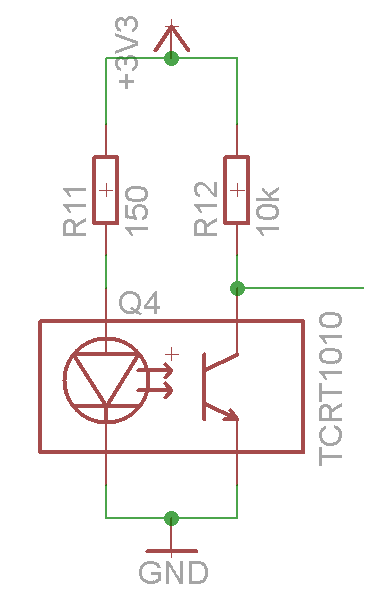
\includegraphics[scale=0.5]{Figures/TCRT_Circuit.png}
\end{figure}

\begin{figure}
\caption{Graph of Wheel Angle against Voltage read by AVR}
\label{Graph:WheelVoltage}
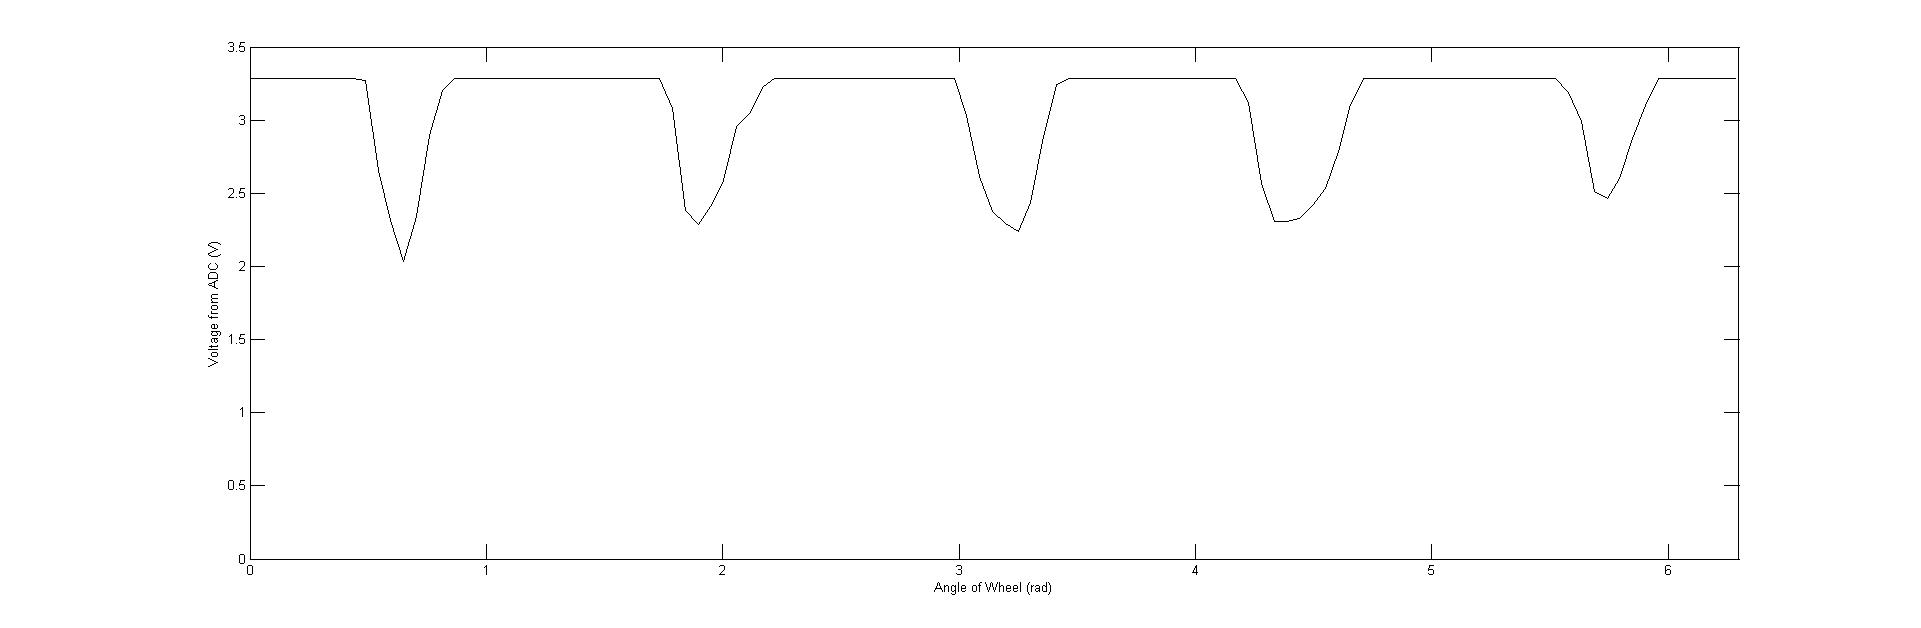
\includegraphics[width = \textwidth]{Figures/WheelVoltageGraph.jpg}
\end{figure}

%\subsubsection{Derivations of Movement Calculations}
%Two basic movements were decided to be implemented: Straight line and rotation. 

\subsubsection{Firmware Development}

As the voltage swing from the phototransistor does not reach 0V the AVR cannot detect this as a logical 0. The internal ADC can be used to continually read the analogue voltage from the phototransistor and detect low points from this data. This method requires the processor to continually compare values and process the data. However, more control would be had over the noise in the data.

An alternative is to use an analogue comparator built in on most AVRs. This can be set up to run an interrupt service routine when the voltage crosses a threshold. The threshold voltage can be determined by a potentiometer. The code is primarily two methods, the set up and the ISR.

Set up is different for if a rotation or movement is wanted. Moving in a straight line takes a parameter of how far to move as a signed integer and calculates the total number of interrupts that need to occur can be calculated using \eqref{eq:NumberInterrupts}. This value is put in a global variable. The PWM and input pins to set the correct direction are then set up before enabling the motor. 

\begin{equation}
\label{eq:NumberInterrupts}
Interrupts = D \times \frac{IPR}{C_w}
\end{equation}

To rotate, one of three methods can be used: Spot rotation on the centre of the robot, or pivot on either left or right wheel. For ease, the Spot rotation is the only one implemented. To calculate the distance moved, the radius to the wheels needs to be known. The circumference through the wheels is then easily calculated and the angle of rotation is then a ratio. The distance to move is calculated by equation \eqref{eq:RotationalDistance} and the total number of interrupts can be calculated using equation \eqref{eq:NumberInterrupts}. To rotate clockwise, the left motor is driven forward and the right is driven backwards. To rotate anti-clockwise, the directions are reversed

\begin{equation}
\label{eq:RotationalDistance}
D_{R} = A \times \frac{C_b}{360}
\end{equation}

Combining equations \eqref{eq:NumberInterrupts} and \eqref{eq:RotationalDistance} gives:
\begin{equation}
\label{eq:RotationalInterrupts}
Interrupts = A \times \frac{IPR}{C_w} \times \frac{C_b}{360}
\end{equation}
Where $A$ is the angle to rotate in degrees, $IPR$ is the number of interrupts generated per full revolution of the wheel, $C_w$ is the circumference of the wheel and $C_b$ the $2\pi\times r_b$ and $r_b$ is the distance from the centre of the robot to the centre of the wheel (see figure \ref{fig:RobotBase_Annotated}).



\begin{figure}
\centering
\subfigure[Top View of robot base showing dimensions of interest\label{fg:RobotBase:Top}]{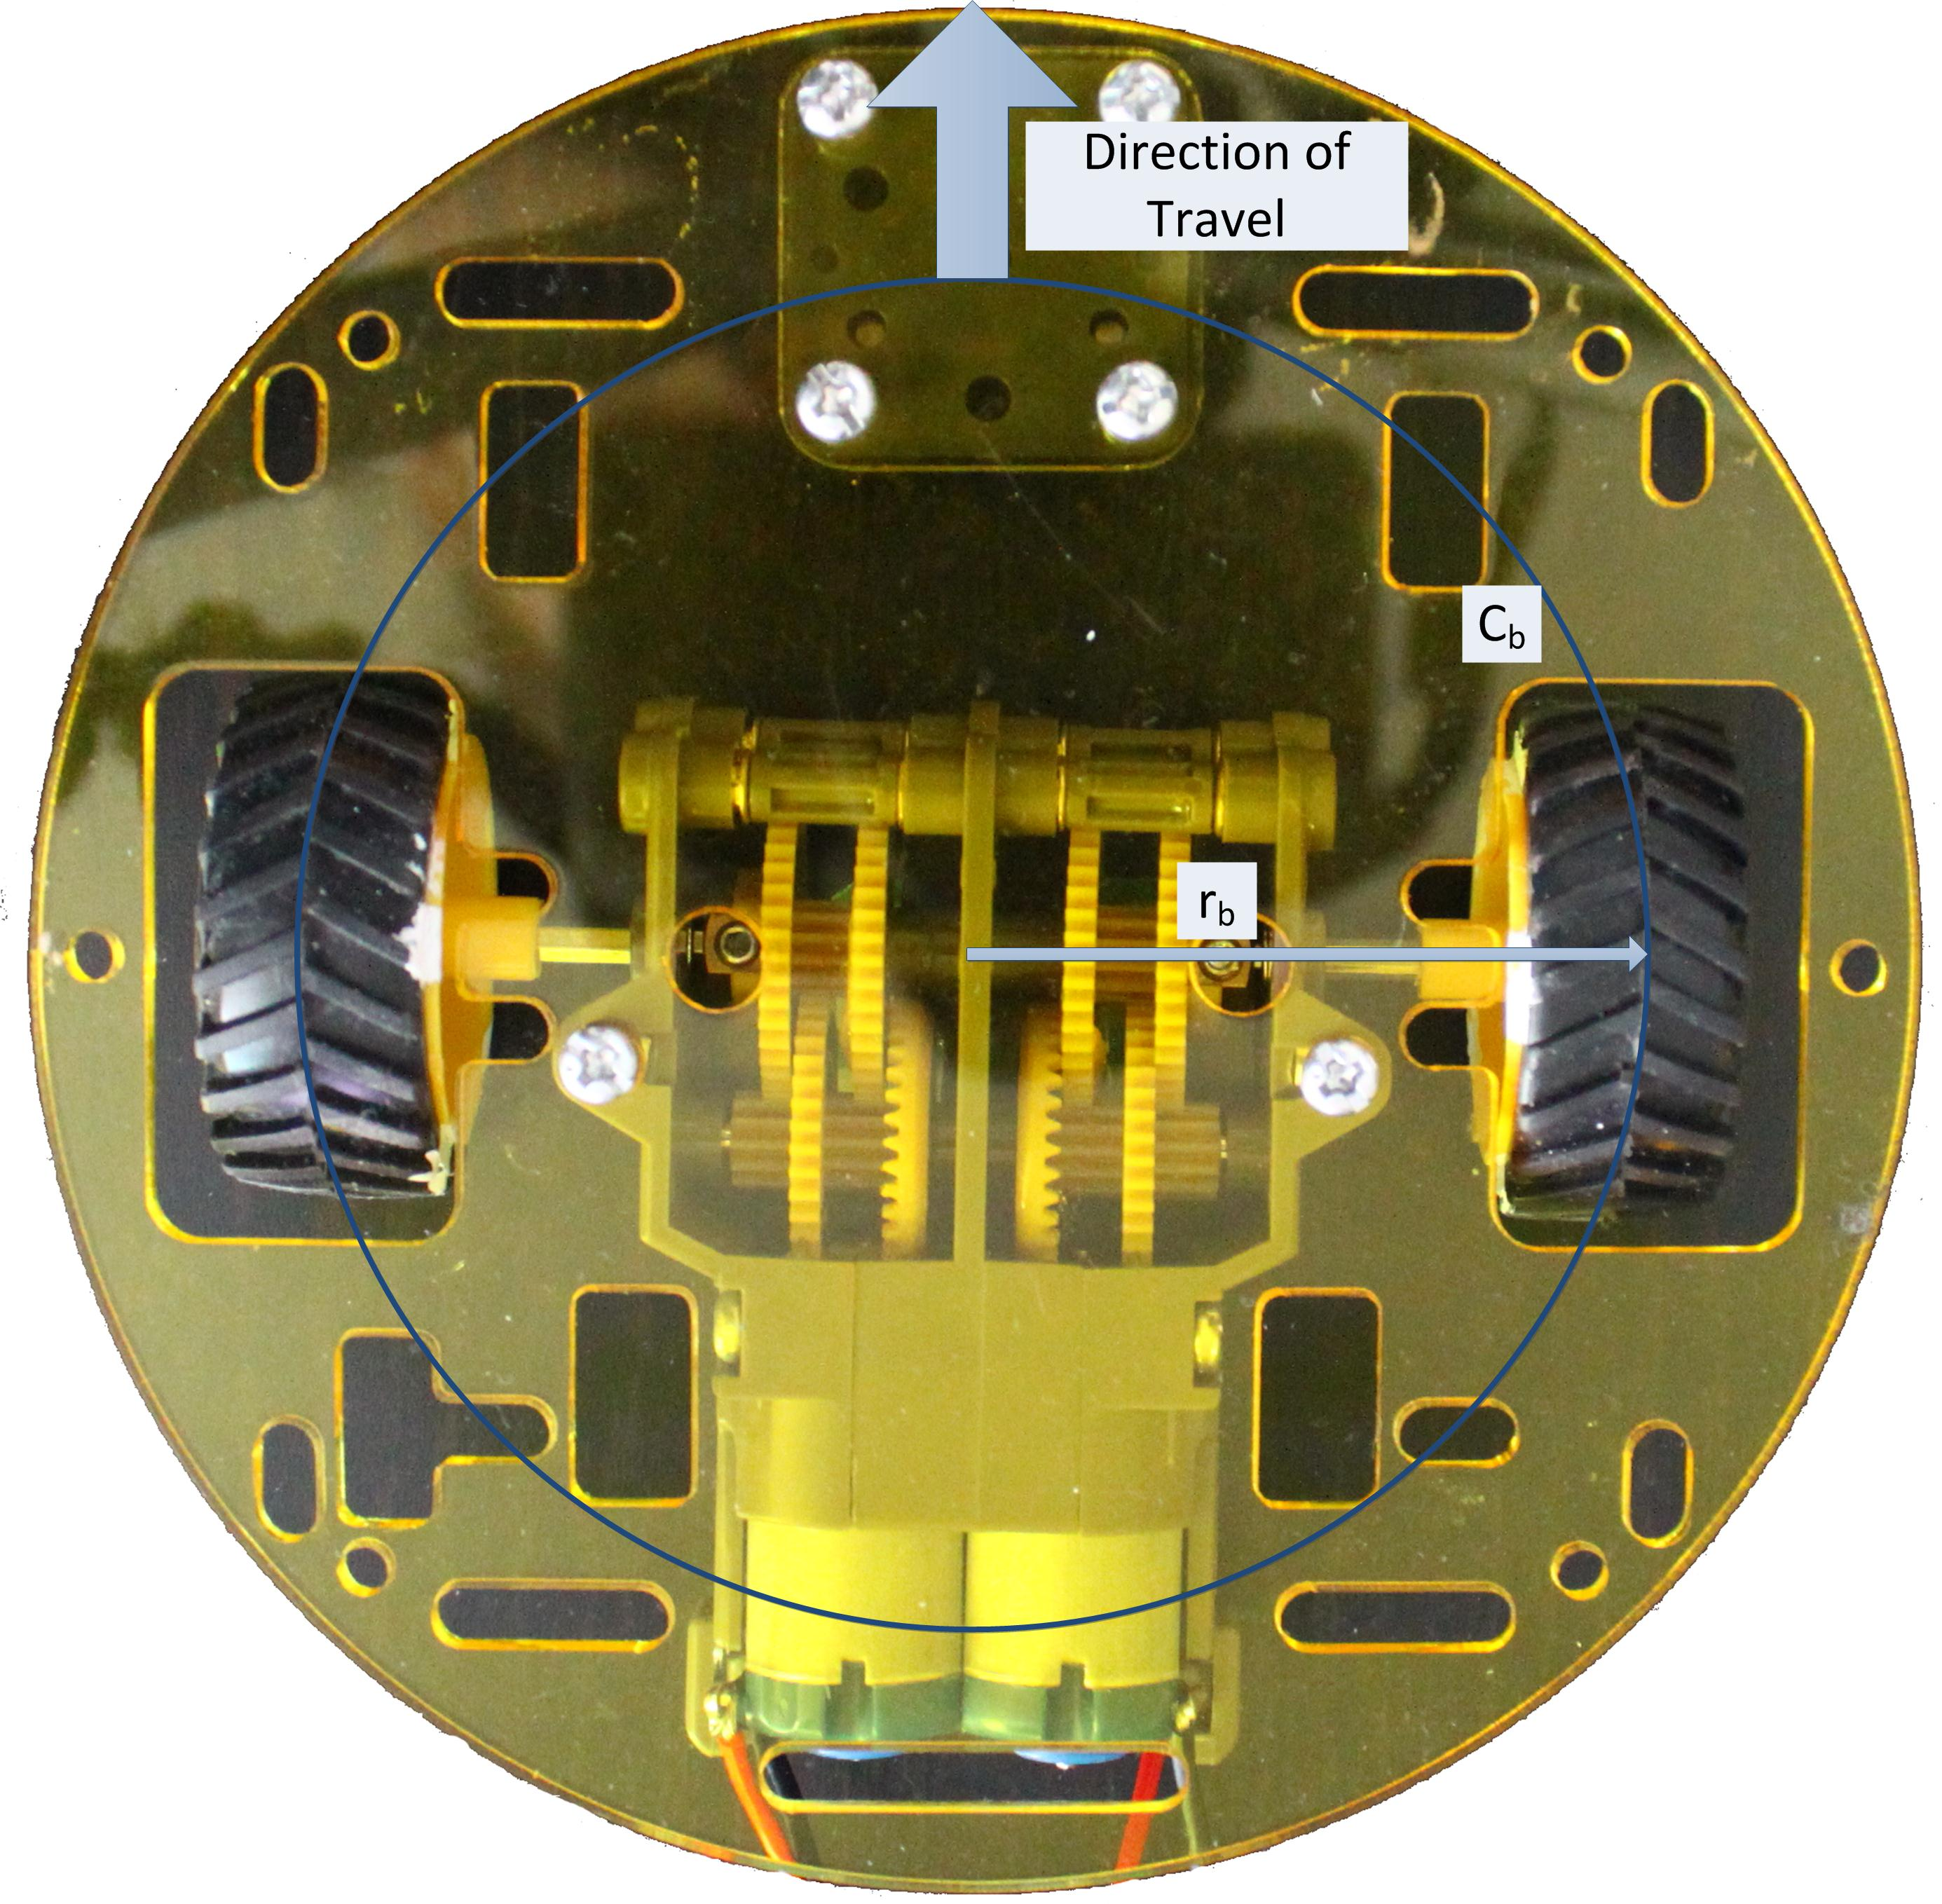
\includegraphics[width = \textwidth, keepaspectratio]{./Figures/Robotbase_top_annot.jpg} }
\subfigure[Side View of robot base showing dimensions of interest\label{fg:RobotBase:Side}]{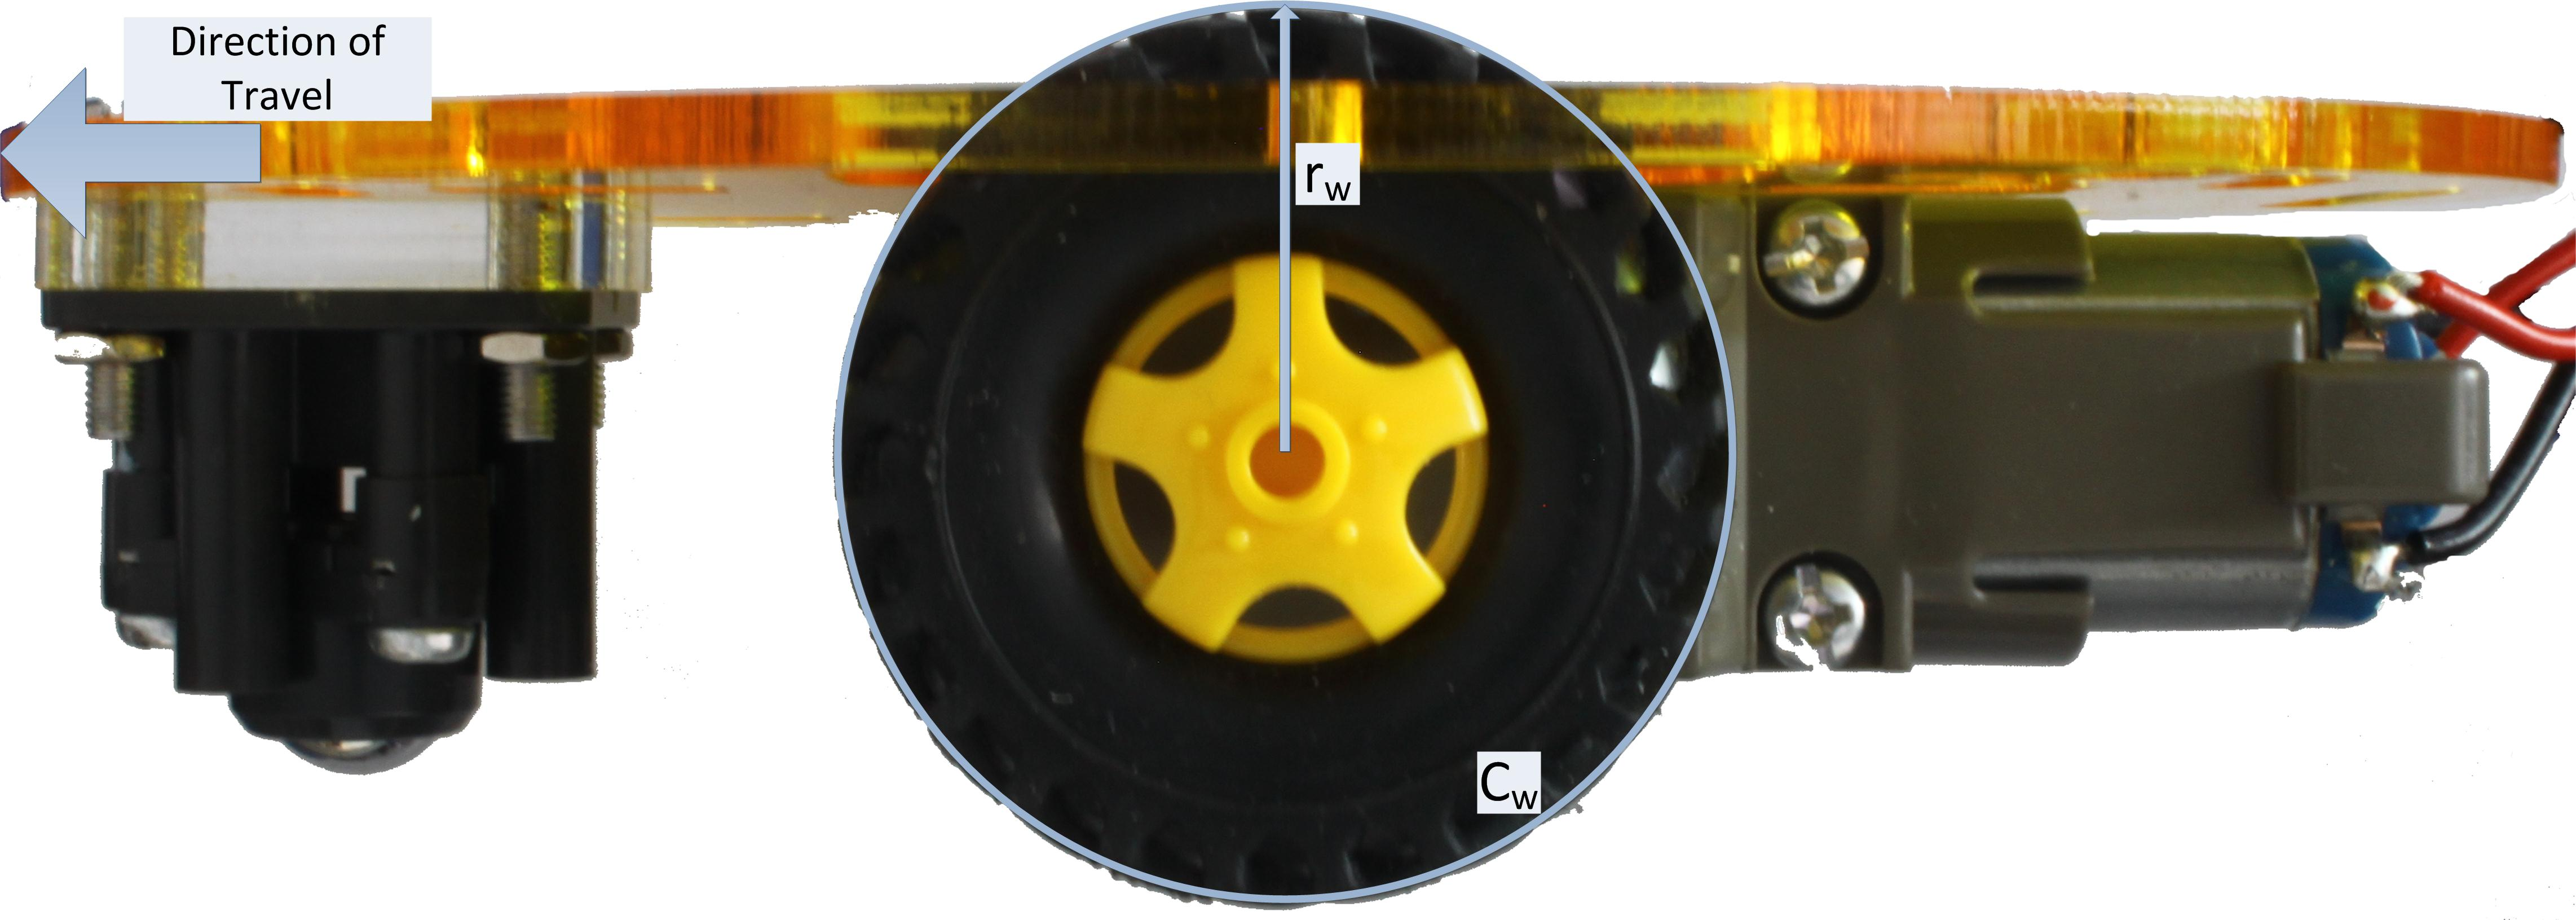
\includegraphics[width = \textwidth, keepaspectratio]{./Figures/Robotbase_side_annot.jpg} }
\caption{Dimensions of Interest for Robot Movement}
\label{fig:RobotBase_Annotated}
\end{figure}
\inote{Maybe a figure to explain better?}


The motor speed can be controlled by Pulse Width Modulation (PWM). The code sets up a low duty cycle PWM signal to drive the motors slowly. This removes the need for a controller to ensure the correct distance was moved. 

The final code can be seen in appendix \ref{Chapter:AppendixC:Code}
\subsubsection{Testing}


\subsubsection{Conclusion}
\section{PCB Development}
\subsection{PCB Design}
\inote{Considerations - Track Equalisation, Power consumption of devices not exceeding VReg}
\inote{Layout}
\inote{Over Engineering?}
\subsection{PCB Testing}
\inote{Building}
\inote{How I tested}
\inote{Problems I found}
\inote{Solutions to the Problems}
\inote{Current Consumption?}
\subsection{PCB Amendments and Conclusion}
\inote{Rev B of the PCB / list of problems}
\inote{Given more time, different}

\section{Conclusions}
\inote{Overall Conclusions of the Hardware design}